\documentclass[11pt]{article}
\usepackage[utf8]{inputenc}
\usepackage{amsmath}
\usepackage{listings}
\usepackage{color}
\usepackage{graphicx}
\graphicspath{ {imagenes/} }

\lstset{
	language=C++,
    basicstyle=\ttfamily,
    keywordstyle=\color{blue}\ttfamily,
    stringstyle=\color{red}\ttfamily,
    commentstyle=\color{green}\ttfamily,
    morecomment=[l][\color{magenta}]{\#}
}

\title{\textbf{El que no es chorro es criminal}}
\author{El pesado}
\date{}
\begin{document}

\maketitle
\newpage
\tableofcontents
\newpage
\section{Estructuras}
\begin{itemize}
\item  Estructura que cuente la cantidad de asistentes de las charlas sin procesar  (valor -2).
\end{itemize}

\begin{itemize}
\item  Estructura que cuente la cantidad de asistentes de las charlas no asignadas a sala (valor -1).
\end{itemize}

\begin{itemize}
\item  Estructura que cuente la cantidad de asistentes de las charlas que han sido jasta el momento asignadas a sala (valor mayor a cero).
\end{itemize}

\begin{itemize}
\item  Tupla solución actual con cantidad de asistentes de la tupla solución.
\end{itemize}


\textbf{Observacion:} Al referime a estructura estoy diciendo que puede ser cualquier cosa, una celda escondida en la tupla o variable global o pasada por parámetro.

\newpage
\section{Recorrida con -2}
Para el caso de la recorrida con valor inicial de tupla -2. 
Tenemos para el caso: 3 \textit{charlas} y 2 \textit{salas}.

\begin{center}
  \makebox[\textwidth]{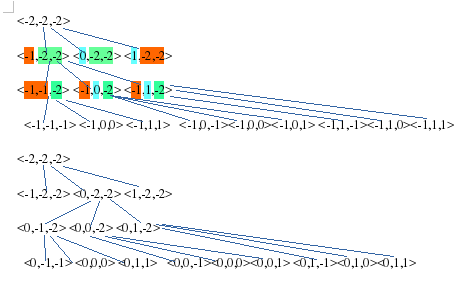
\includegraphics{recorrido}}
\end{center}

Hasta llegar a las hojas tenemos que muchos casos repiten cierto patrón.

\begin{enumerate}
\item Hay un conjunto de charlas  {\color{green} \textit{sin procesar}}  y hay un conjunto de charlas {\color{red} \textit{sin asignar}} .

\item Hay un conjunto de charlas sin {\color{green} \textit{procesar}}, hay un conjunto de charlas {\color{red} \textit{sin asignar}} y hay una charla {\color{blue} \textit{ya asignada}}  .

\end{enumerate}

\section{Propuesta: (ruido)}
Meditarlo en el viaje



\end{document}
